\chapter{Experimentaci\'{o}n}

En este cap\'{i}tulo mostraremos el rendimiento de la mejor versi\'{o}n implementada, la tercera versi\'{o}n, aquella con la <<secci\'{o}n critica mejorada>> y haciendo uso de la malla de \textit{locks} con m\'{a}s detalle. En las anteriores presentaciones de los rendimientos de las distintas implementaciones se ha utilizado un tipo concreto de imagen, con un tama\~{n}o determinado (3000x2800) y una inicializaci\'{o}n espec\'{i}fica del contorno. En este apartado realizaremos pruebas m\'{a}s completas, combinando distintos factores para ver m\'{a}s detalladamente el comportamiento de la mejor versi\'{o}n de la paralela. Adem\'{a}s, se podr\'{a} llegar a concluir qu\'{e} tipo de combinaci\'{o}n beneficia a la evoluci\'{o}n del contorno en cierto tipo de im\'{a}genes.

Se ha decidido probar 3 tipos de im\'{a}genes diferentes, con varios tama\~{n}os de \'{e}stas, varios tama\~{n}os de las mallas de \textit{locks} y varios \textit{threads}. En la figura \ref{tiposImagenes} se puede observar los tres tipos de im\'{a}genes diferentes que se utilizar\'{a}n en la realizaci\'{o}n de dichas pruebas.


\begin{figure}[H]
	\centering	
	\captionsetup{justification=centering}	
	\begin{center}
		\begin{subfigure}[t]{2.5in}
			\centering
			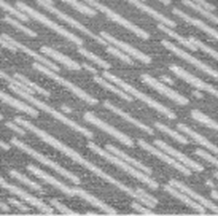
\includegraphics[width=.7\textwidth]{./imagenes/buena1}
			\subcaption{}\label{buena1}
		\end{subfigure}
		\begin{subfigure}[t]{2.5in}
			\centering
			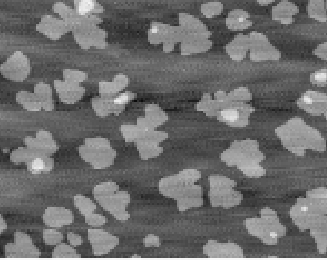
\includegraphics[width=.8\textwidth]{./imagenes/ejemplo2}	
			\subcaption{}\label{buena2}
		\end{subfigure}
		\begin{subfigure}[t]{2.5in}
			\centering
			
\includegraphics[width=.8\textwidth]{./imagenes/buena3}	
			\subcaption{}\label{buena3}
		\end{subfigure}
	\end{center}
	\caption{Tipos de im\'{a}genes con las que se realizar\'{a}n las pruebas completas de la tercera implementaci\'{o}n}
	\label{tiposImagenes}
\end{figure} 


\section{Primera imagen}

La primera imagen a probar ser\'{a} la imagen \ref{buena1}, una imagen borrosa, con poca diferencia en tono de gris entre las islas y el fondo, y con una morfolog\'{i}a de las islas alargada. A continuaci\'{o}n se presentan los resultados de las ejecuciones con diferentes tama\~{n}os de la imagen. Se ha resaltado en negrita el mejor tiempo de ejecuci\'{o}n y se ha marcado con un asterisco los valores m\'{a}s cercano al \'{o}ptimo conseguido.

\subsubsection{500x500}

\begin{table}[H]
	\centering
	\small
	\begin{tabular}{|c|c|c|c|c|c|c|}
		\hline
		{\bf \backslashbox{Threads}{Locks}}   & {\bf 4} & {\bf 8} & {\bf 16} & {\bf 24} & {\bf 32} & {\bf 50} \\ \hline
		{\bf Serie}  & 2,01    & 2,03    & 2,03     & 2,04     & 2,04     & 2,03     \\ \hline
		{\bf 2}  & 1,34    & 1,37    & 1,37     & 1,34     & 1,35     & 1,35     \\ \hline
		{\bf 4}  & 1,00    & 0,96    & 0,96     & 0,97     & 0,96     & 0,95     \\ \hline
		{\bf 8}  & 0,62    & 0,91    & 0,91     & 0,80     & 0,88     & 0,90     \\ \hline
		{\bf 12} & 0,62    & 0,72    & 0,72     & 0,64     & 0,81     & 0,81     \\ \hline
		{\bf 16} & 0,62    & 0,56    & 0,56     & 0,48     & 0,74     & 0,70     \\ \hline
		{\bf 20} & 0,53    & 0,64    & 0,64     & 0,50     & 0,67     & 0,60     \\ \hline
		{\bf 24} & 0,43    & 0,52    & 0,52     & 0,56     & 0,56     & 0,49     \\ \hline
		{\bf 28} & 0,47    & 0,43    & 0,43     & 0,45     & 0,43     & 0,47     \\ \hline
		{\bf 32} & 0,42    & 0,40    & 0,40     & 0,39     & 0,38     & 0,39     \\ \hline
		{\bf 36} & 0,44    & 0,37    & 0,37     & 0,35     & 0,34     & 0,36     \\ \hline
		{\bf 40} & 0,44    & 0,32    & 0,32     & 0,31*     & 0,32     & 0,32     \\ \hline
		{\bf 44} & 0,45    & 0,35    & 0,35     & 0,31*     & 0,31*     & \textbf{0,30}     \\ \hline
		{\bf 48} & 0,45    & 0,36    & 0,36     & 0,33     & 0,34     & 0,37     \\ \hline
	\end{tabular}
	\captionsetup{justification=centering}	
	\caption{Tiempos de ejecuci\'{o}n (s) de la imagen \ref{buena1} con un tama\~{n}o de 500x500}
	\label{img1-500}	
\end{table}

Como se puede observar en la tabla \ref{img1-500} los mejores tiempos se consiguen con 40 y 44 \textit{threads} y a partir de los 24 \textit{locks}. El menor tiempo que se consigue es de 0,3 segundos, con un \textit{speed-up} de 6,7 y una eficiencia del 15,1\%.

\begin{figure}[H]
	\captionsetup{justification=centering}
	\centering
	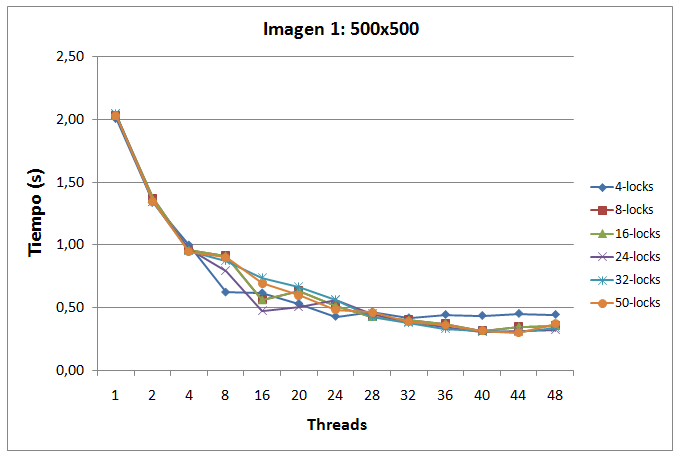
\includegraphics[width=.7\textwidth]{./imagenes/graf1-500}
	\caption{Gr\'{a}fica de los tiempos de ejecuci\'{o}n de la imagen \ref{buena1} con un tama\~{n}o de 500x500}	
	\label{graf1-500}
\end{figure}

\subsubsection{1500x1500}


\begin{table}[H]
	\centering
	\small
	\begin{tabular}{|c|c|c|c|c|c|c|}
		\hline
		{\bf \backslashbox{Threads}{Locks}}   & {\bf 4} & {\bf 8} & {\bf 16} & {\bf 24} & {\bf 32} & {\bf 50} \\ \hline
		{\bf Serie}  & 14,88   & 14,91   & 14,92    & 14,87    & 14,92    & 14,90    \\ \hline
		{\bf 2}  & 8,52    & 8,54    & 8,42     & 8,54     & 8,52     & 8,50     \\ \hline
		{\bf 4}  & 5,96    & 5,96    & 5,82     & 5,88     & 5,88     & 5,88     \\ \hline
		{\bf 8}  & 3,34    & 4,89    & 4,87     & 4,80     & 4,80     & 4,80     \\ \hline
		{\bf 12} & 3,40    & 4,10    & 4,51     & 3,68     & 4,59     & 4,51     \\ \hline
		{\bf 16} & 3,45    & 3,40    & 4,27     & 2,58     & 4,28     & 4,27     \\ \hline
		{\bf 20} & 2,86    & 3,50    & 3,51     & 2,72     & 3,43     & 3,43     \\ \hline
		{\bf 24} & 2,34    & 2,89    & 2,90     & 2,87     & 2,86     & 2,86     \\ \hline
		{\bf 28} & 2,63    & 2,50    & 2,52     & 2,50     & 2,47     & 2,49     \\ \hline
		{\bf 32} & 2,65    & 2,28    & 2,23     & 2,27     & 2,23     & 2,26     \\ \hline
		{\bf 36} & 2,64    & 2,10    & 2,20     & 2,19     & 2,21     & 2,23     \\ \hline
		{\bf 40} & 2,69    & 2,16    & 2,17     & 2,17     & 2,16     & 2,16     \\ \hline
		{\bf 44} & 2,66    & 2,05    & 2,07     & 2,08     & 2,06     & 2,05*     \\ \hline
		{\bf 48} & 2,79    & 2,14    & 2,05*     & 2,05*     & 2,07     & \textbf{2,02}     \\ \hline
	\end{tabular}
	\captionsetup{justification=centering}	
	\caption{Tiempos de ejecuci\'{o}n (s) de la imagen \ref{buena1} con un tama\~{n}o de 1500x1500}
	\label{img1-1500}
\end{table}

En esta ocasi\'{o}n el mejor resultado se consigue con 48 \textit{threads} y 50 \textit{locks}. El resultado obtenido son 2,02 segundos,  un \textit{speed-up} de 7,4 y una eficiencia del 15,4\%.


\begin{figure}[H]
	\captionsetup{justification=centering}
	\centering
	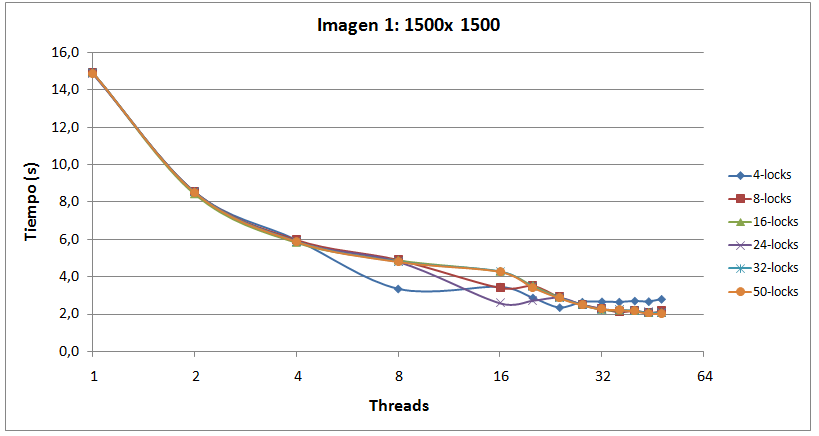
\includegraphics[width=.9\textwidth]{./imagenes/graf1-1500}
	\caption{Gr\'{a}fica de los tiempos de ejecuci\'{o}n de la imagen \ref{buena1} con un tama\~{n}o de 1500x1500}	
	\label{graf1-1500}
\end{figure}

\subsubsection{3000x3000}

\begin{table}[H]
	\centering
	\small
	\begin{tabular}{|c|c|c|c|c|c|c|}
		\hline
		{\bf }   & {\bf 4} & {\bf 8} & {\bf 16} & {\bf 24} & {\bf 32} & {\bf 50} \\ \hline
		{\bf Serie}  & 43,38   & 43,28   & 43,32    & 43,34    & 43,24    & 43,19    \\ \hline
		{\bf 2}  & 28,46   & 26,85   & 26,83    & 26,89    & 26,75    & 26,71    \\ \hline
		{\bf 4}  & 16,94   & 17,25   & 17,18    & 17,00    & 16,99    & 16,80    \\ \hline
		{\bf 8}  & 9,53    & 13,34   & 13,42    & 13,42    & 13,34    & 13,38    \\ \hline
	    {\bf 12} & 9,56    & 11,42   & 12,71    & 10,35    & 12,61    & 12,74    \\ \hline
		{\bf 16} & 9,59    & 9,50    & 12,01    & 7,36     & 11,98    & 12,00    \\ \hline
		{\bf 20} & 7,85    & 9,69    & 9,71     & 7,77     & 9,67     & 9,76     \\ \hline
		{\bf 24} & 6,81    & 8,30    & 8,29     & 8,25     & 8,20     & 8,24     \\ \hline
		{\bf 28} & 7,42    & 7,19    & 7,22     & 7,18     & 7,13     & 7,19     \\ \hline
		{\bf 32} & 7,55    & 7,06    & 7,03     & 7,04     & 6,98     & 6,83     \\ \hline
		{\bf 36} & 7,75    & 6,90    & 7,10     & 7,22     & 7,19     & 6,97     \\ \hline
		{\bf 40} & 8,00    & 7,05    & 6,93     & 6,91     & 6,90     & 6,88     \\ \hline
		{\bf 44} & 8,17    & 6,62    & 6,64     & 6,63     & 6,78     & 6,72     \\ \hline
		{\bf 48} & 8,02    & 6,64    & 6,52*     & \textbf{6,49}     & 6,75     & 6,58     \\ \hline
	\end{tabular}
	\captionsetup{justification=centering}	
	\caption{Tiempos de ejecuci\'{o}n (s) de la imagen \ref{buena1} con un tama\~{n}o de 3000x3000}
	\label{img1-3000}
\end{table}

El mejor resultado es de 6,49 y se alcanza con 48 \textit{threads} y 24 \textit{locks}. Se obtiene un \textit{speed-up} de 6,7 y una eficiencia del 13,9\%.

\begin{figure}[H]
	\captionsetup{justification=centering}
	\centering
	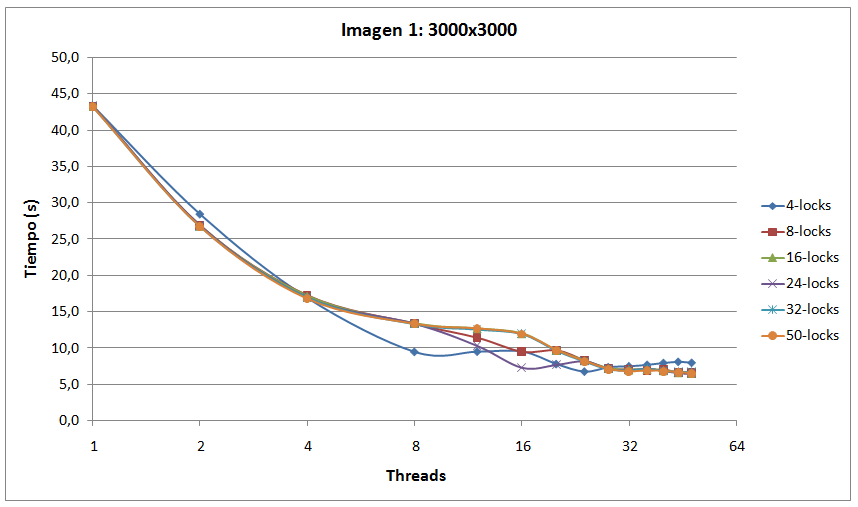
\includegraphics[width=.9\textwidth]{./imagenes/graf1-3000}
	\caption{Gr\'{a}fica de los tiempos de ejecuci\'{o}n de la imagen \ref{buena1} con un tama\~{n}o de 3000x3000}	
	\label{graf1-3000}
\end{figure}

\subsubsection{Resultado}


Los resultados de la segmentaci\'{o}n de esta primera imagen han sido los que se muestran en \ref{result1}, donde se ha marcado la lista $L_{out}$ de color rojo y la lista $L_{in}$ de azul. Se ha conseguido obtener el contorno las islas que es lo que se esperaba.


\begin{figure}[H]
	\captionsetup{justification=centering}
	\centering
	
\includegraphics[width=.7\textwidth]{./imagenes/result1}
	\caption{Resultado de la segmentaci\'{o}n de la imagen \ref{buena1} con un tama\~{n}o de 3000x3000}	
	\label{result1}
\end{figure}


\section{Segunda imagen}

La segunda imagen a probar ser\'{a} la imagen \ref{buena2}. Esta imagen tiene un contraste mayor que la anterior entre la isla y el fondo. La morfolog\'{i}a de las islas es amorfa y algunas tienen peque\~{n}os huecos. Las islas tambi\'{e}n tienen un tama\~{n}o m\'{a}s grande. A continuaci\'{o}n se presentan los resultados de las ejecuciones con diferentes tama\~{n}os de la imagen. Se ha resaltado en negrita el mejor tiempo de ejecuci\'{o}n y se ha marcado con un asterisco los valores m\'{a}s cercano al \'{o}ptimo conseguido.

\subsubsection{500x500}

\begin{table}[H]
	\centering
	\small
	\begin{tabular}{|c|c|c|c|c|c|c|}
		\hline
		{\bf \backslashbox{Threads}{Locks}}   & {\bf 4} & {\bf 8} & {\bf 16} & {\bf 24} & {\bf 32} & {\bf 50} \\ \hline
		{\bf Serie}  & 0,51    & 0,51    & 0,52     & 0,51     & 0,51     & 0,52     \\ \hline
		{\bf 2}  & 0,35    & 0,35    & 0,35     & 0,35     & 0,34     & 0,34     \\ \hline
		{\bf 4}  & 0,25    & 0,25    & 0,25     & 0,25     & 0,24     & 0,24     \\ \hline
		{\bf 8}  & 0,17    & 0,21    & 0,21     & 0,20     & 0,20     & 0,20     \\ \hline
		{\bf 12} & 0,17    & 0,18    & 0,19     & 0,17     & 0,19     & 0,19     \\ \hline
		{\bf 16} & 0,16    & 0,15    & 0,18     & 0,13     & 0,18     & 0,18     \\ \hline
		{\bf 20} & 0,13    & 0,15    & 0,15     & 0,13     & 0,15     & 0,15     \\ \hline
		{\bf 24} & 0,13    & 0,14    & 0,13     & 0,13     & 0,13     & 0,13     \\ \hline
		{\bf 28} & 0,16    & 0,12    & 0,12     & 0,12     & 0,12     & 0,12     \\ \hline
		{\bf 32} & 0,17    & 0,11    & 0,11     & 0,11     & 0,11     & 0,11     \\ \hline
		{\bf 36} & 0,18    & 0,12    & 0,11     & 0,11     & 0,11     & 0,11     \\ \hline
		{\bf 40} & 0,20    & 0,11    & 0,11     & \textbf{0,10}     & \textbf{0,10}     & 0,11     \\ \hline
		{\bf 44} & 0,21    & 0,13    & 0,11     & 0,11     & \textbf{0,10}     & \textbf{0,10}     \\ \hline
		{\bf 48} & 0,23    & 0,18    & 0,14     & 0,13     & 0,14     & 0,15     \\ \hline
	\end{tabular}
	\captionsetup{justification=centering}	
	\caption{Tiempos de ejecuci\'{o}n (s) de la imagen \ref{buena2} con un tama\~{n}o de 500x500}
	\label{img2-500}
\end{table}

Como se puede observar en la tabla \ref{img2-500} los mejores tiempos se consiguen con 40 y 44 \textit{threads} y a partir de los 24 \textit{locks}. El menor tiempo que se consigue es de 0,10 segundos, con un \textit{speed-up} de 4,9 y una eficiencia del 12,5\%.

\begin{figure}[H]
	\captionsetup{justification=centering}
	\centering
	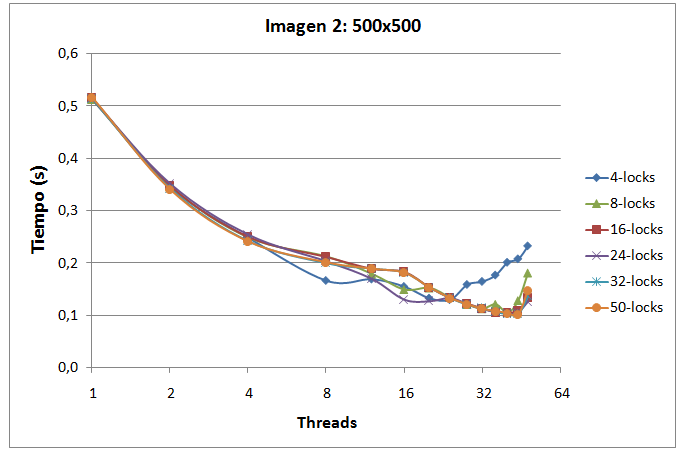
\includegraphics[width=.7\textwidth]{./imagenes/graf2-500}
	\caption{Gr\'{a}fica de los tiempos de ejecuci\'{o}n de la imagen \ref{buena2} con un tama\~{n}o de 500x500}	
	\label{graf2-500}
\end{figure}


\subsubsection{1500x1500}

\begin{table}[H]
	\centering
	\small
	\begin{tabular}{|c|c|c|c|c|c|c|}
		\hline
		{\bf \backslashbox{Threads}{Locks}}   & {\bf 4} & {\bf 8} & {\bf 16} & {\bf 24} & {\bf 32} & {\bf 50} \\ \hline
		{\bf Serie}  & 5,45    & 5,45    & 5,46     & 5,47     & 5,46     & 5,46     \\ \hline
		{\bf 2}  & 3,56    & 3,61    & 3,57     & 3,56     & 3,54     & 3,54     \\ \hline
		{\bf 4}  & 2,63    & 2,67    & 2,65     & 2,58     & 2,58     & 2,56     \\ \hline
		{\bf 8}  & 1,68    & 2,23    & 2,20     & 2,11     & 2,11     & 2,10     \\ \hline
		{\bf 12} & 1,61    & 1,89    & 2,00     & 1,65     & 1,65     & 1,97     \\ \hline
		{\bf 16} & 1,55    & 1,50    & 1,82     & 1,22     & 1,22     & 1,83     \\ \hline
		{\bf 20} & 1,31    & 1,53    & 1,53     & 1,21     & 1,23     & 1,53     \\ \hline
		{\bf 24} & 1,15    & 1,31    & 1,31     & 1,30     & 1,31     & 1,32     \\ \hline
		{\bf 28} & 1,43    & 1,17    & 1,19     & 1,18     & 1,19     & 1,17     \\ \hline
		{\bf 32} & 1,59    & 1,12*    & 1,12*     & 1,12*     & 1,13     & \textbf{1,10}     \\ \hline
		{\bf 36} & 1,82    & 1,27    & 1,26     & 1,24     & 1,27     & 1,31     \\ \hline
		{\bf 40} & 1,97    & 1,37    & 1,39     & 1,40     & 1,37     & 1,35     \\ \hline
		{\bf 44} & 2,03    & 1,40    & 1,38     & 1,41     & 1,36     & 1,39     \\ \hline
		{\bf 48} & 2,16    & 1,80    & 1,41     & 1,37     & 1,42     & 1,42     \\ \hline
	\end{tabular}
	\captionsetup{justification=centering}	
	\caption{Tiempos de ejecuci\'{o}n (s) de la imagen \ref{buena2} con un tama\~{n}o de 1500x1500}
	\label{img2-1500}
\end{table}

Como se puede observar en la tabla \ref{img2-1500} el mejor resultado obtenido es de 1,10 segundos, con la combinaci\'{o}n de 32 \textit{threads} y 50 \textit{locks}. Se consigue por lo tanto un \textit{speed-up} de 4,9 y una eficiencia del 15,5\%. 

\begin{figure}[H]
	\captionsetup{justification=centering}
	\centering
	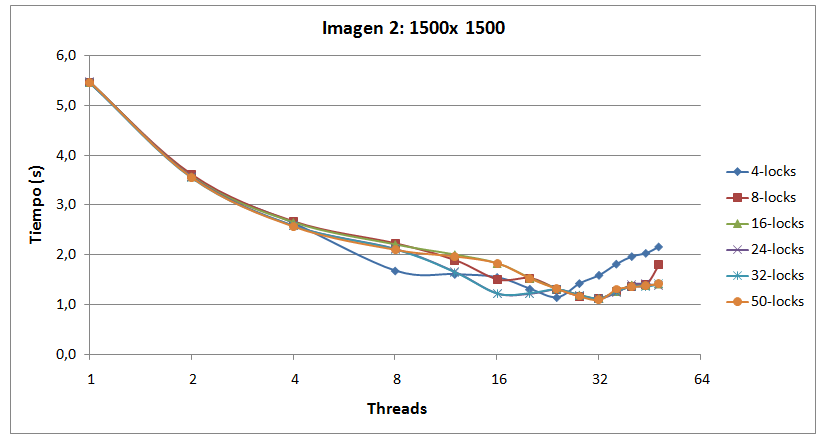
\includegraphics[width=.9\textwidth]{./imagenes/graf2-1500}
	\caption{Gr\'{a}fica de los tiempos de ejecuci\'{o}n de la imagen \ref{buena2} con un tama\~{n}o de 1500x1500}	
	\label{graf2-1500}
\end{figure}


\subsubsection{3000x3000}

\begin{table}[H]
	\centering
	\small
	\begin{tabular}{|c|c|c|c|c|c|c|}
		\hline
		{\bf \backslashbox{Threads}{Locks}}   & {\bf 4} & {\bf 8} & {\bf 16} & {\bf 24} & {\bf 32} & {\bf 50} \\ \hline
		{\bf Serie}  & 22,29   & 22,40   & 22,25    & 22,29    & 22,27    & 22,31    \\ \hline
		{\bf 2}  & 9,64    & 9,65    & 9,83     & 9,61     & 9,58     & 9,58     \\ \hline
		{\bf 4}  & 12,42   & 12,41   & 12,64    & 12,20    & 12,21    & 12,06    \\ \hline
		{\bf 8}  & 5,88    & 7,57    & 7,61     & 7,65     & 7,53     & 7,54     \\ \hline
		{\bf 12} & 5,74    & 6,51    & 7,24     & 6,01     & 7,12     & 7,13     \\ \hline
		{\bf 16} & 5,67    & 5,43    & 6,74     & 4,48     & 6,71     & 6,72     \\ \hline
		{\bf 20} & 4,62    & 5,45    & 5,49     & 4,50     & 5,50     & 5,49     \\ \hline
		{\bf 24} & 4,07    & 4,69    & 4,72     & 4,67     & 4,66     & 4,66     \\ \hline
		{\bf 28} & 4,50    & 4,16    & 4,27     & 4,27     & 4,13*     & 4,10*     \\ \hline
		{\bf 32} & 5,08    & 4,34    & 4,15     & 4,58     & \textbf{3,85}     & 3,89*     \\ \hline
		{\bf 36} & 6,14    & 4,72    & 5,03     & 4,95     & 5,16     & 5,27     \\ \hline
		{\bf 40} & 6,65    & 5,22    & 5,25     & 5,28     & 5,25     & 5,22     \\ \hline
		{\bf 44} & 7,02    & 5,25    & 5,23     & 5,42     & 5,19     & 5,24     \\ \hline
		{\bf 48} & 7,19    & 5,45    & 5,31     & 5,23     & 5,17     & 5,39     \\ \hline
	\end{tabular}
	\captionsetup{justification=centering}	
	\caption{Tiempos de ejecuci\'{o}n (s) de la imagen \ref{buena2} con un tama\~{n}o de 3000x3000}
	\label{img2-3000}
\end{table}

Como se puede observar en la tabla \ref{img2-3000} el mejor resultado se obtienen con 32 \textit{threads} y a partir de los 32 \textit{locks}. El mejor resultado es de 3,85 segundos, con un \textit{speed-up} de 5,7 y una eficiencia del 18,0\%.  

\begin{figure}[H]
	\captionsetup{justification=centering}
	\centering
	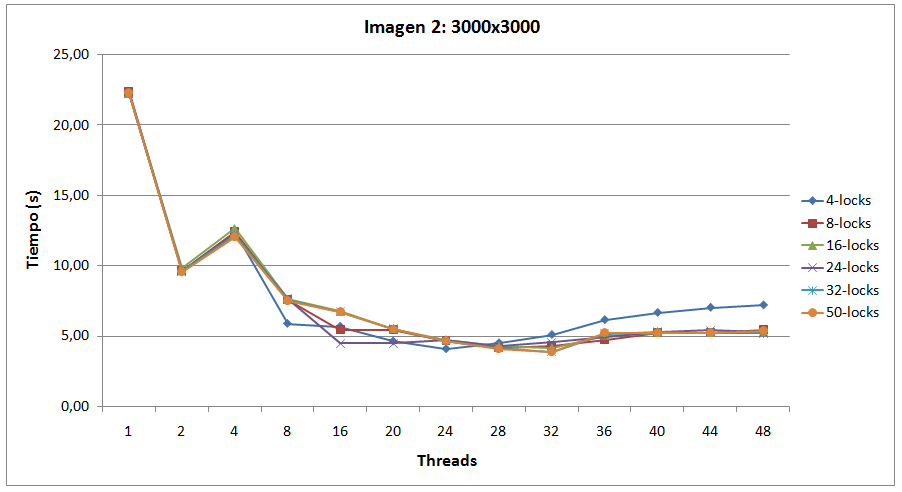
\includegraphics[width=.9\textwidth]{./imagenes/graf2-3000}
	\caption{Gr\'{a}fica de los tiempos de ejecuci\'{o}n de la imagen \ref{buena2} con un tama\~{n}o de 3000x3000}	
	\label{graf2-3000}
\end{figure}


\subsubsection{Resultado}


Los resultados de la segmentaci\'{o}n de esta segunda imagen han sido los que se muestran en \ref{result2}, donde se ha marcado la lista $L_{out}$ de color rojo y la lista $L_{in}$ de azul. Se ha conseguido obtener el contorno las islas que es lo que se esperaba.


\begin{figure}[H]
	\captionsetup{justification=centering}
	\centering
	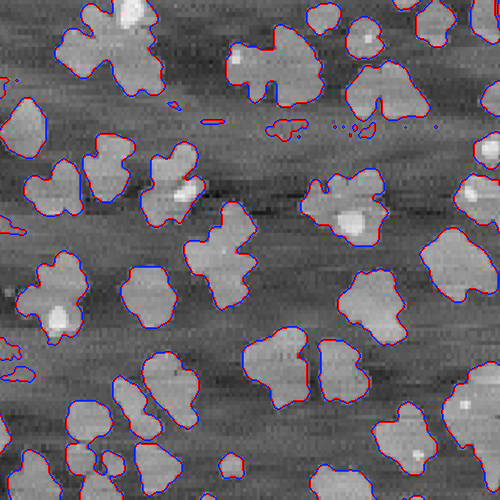
\includegraphics[width=.7\textwidth]{./imagenes/result2}
	\caption{Resultado de la segmentaci\'{o}n de la imagen \ref{buena2} con un tama\~{n}o de imagen de 3000x3000}	
	\label{result2}
\end{figure}


\section{Tercera imagen}

La tercera imagen a probar ser\'{a} la imagen \ref{buena3} y a continuaci\'{o}n se presentan los resultados de las ejecuciones con diferentes tama\~{n}os de la imagen. Esta imagen tiene m\'{a}s contraste entre el fondo y las islas que la anterior ya que es pr\'{a}cticamente binaria. Morfol\'{o}gicamente las islas son menos redondeadas y tienen a\'{u}n m\'{a}s grietas comparadas con las de la anterior imagen. Se ha resaltado en negrita el mejor tiempo de ejecuci\'{o}n y se ha marcado con un asterisco los valores m\'{a}s cercano al \'{o}ptimo conseguido.

\subsubsection{Tama\~{n}o 500x500}

\begin{table}[H]
	\centering
	\small
	\begin{tabular}{|c|c|c|c|c|c|c|}
		\hline
		{\bf \backslashbox{Threads}{Locks}}   & {\bf 4} & {\bf 8} & {\bf 16} & {\bf 24} & {\bf 32} & {\bf 50} \\ \hline
		{\bf Serie}  & 0,72    & 0,73    & 0,72     & 0,73     & 0,72     & 0,72     \\ \hline
		{\bf 2}  & 0,48    & 0,48    & 0,48     & 0,48     & 0,48     & 0,48     \\ \hline
		{\bf 4}  & 0,34    & 0,34    & 0,34     & 0,35     & 0,33     & 0,33     \\ \hline
		{\bf 8}  & 0,21    & 0,28    & 0,28     & 0,27     & 0,27     & 0,27     \\ \hline
		{\bf 12} & 0,21    & 0,24    & 0,26     & 0,23     & 0,26     & 0,26     \\ \hline
		{\bf 16} & 0,20    & 0,19    & 0,24     & 0,16     & 0,24     & 0,24     \\ \hline
		{\bf 20} & 0,17    & 0,20    & 0,20     & 0,16     & 0,20     & 0,20     \\ \hline
		{\bf 24} & 0,15    & 0,17    & 0,17     & 0,17     & 0,17     & 0,17     \\ \hline
		{\bf 28} & 0,17    & 0,15    & 0,15     & 0,15     & 0,15     & 0,15     \\ \hline
		{\bf 32} & 0,17    & 0,14    & 0,14     & 0,14     & 0,14     & 0,14     \\ \hline
		{\bf 36} & 0,18    & 0,14    & 0,13     & 0,13     & 0,13     & 0,13     \\ \hline
		{\bf 40} & 0,19    & 0,12    & 0,13     & \textbf{0,12 }    & \textbf{0,12}     & \textbf{0,12}     \\ \hline
		{\bf 44} & 0,19    & 0,14    & \textbf{0,12}     & \textbf{0,12}     & \textbf{0,12}     & \textbf{0,12 }    \\ \hline
		{\bf 48} & 0,22    & 0,18    & 0,14     & 0,14     & 0,13     & 0,17     \\ \hline
	\end{tabular}
	\captionsetup{justification=centering}	
	\caption{Tiempos de ejecuci\'{o}n (s) de la imagen \ref{buena3} con un tama\~{n}o de 500x500}
	\label{img3-500}
\end{table}

Como se puede observar en la tabla \ref{img3-500} los mejores resultados se consiguen con 40 y 44 \textit{threads} y con mas de 8 \textit{locks}, logrando as\'{i} un tiempo de 0,12 segundos, un \textit{speed-up} de 5,8 y una eficiencia del 14,6\%. 

\begin{figure}[H]
	\captionsetup{justification=centering}
	\centering
	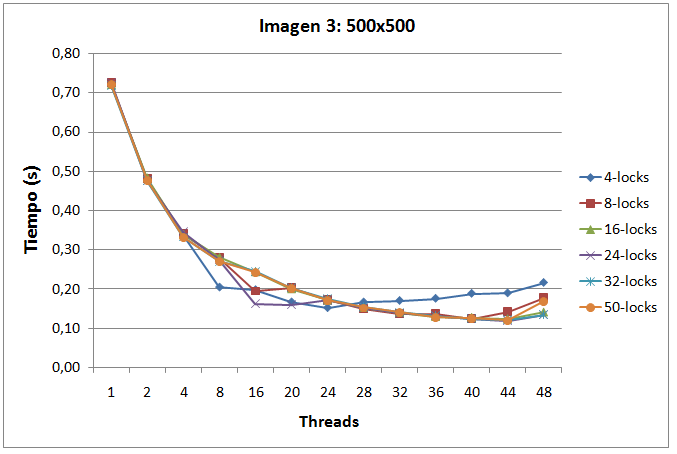
\includegraphics[width=.7\textwidth]{./imagenes/graf3-500}
	\caption{Gr\'{a}fica de los tiempos de ejecuci\'{o}n de la imagen \ref{buena3} con un tama\~{n}o de 500x500}	
	\label{graf3-500}
\end{figure}


\subsubsection{Tama\~{n}o 1500x1500}

\begin{table}[H]
	\centering
	\small
	\begin{tabular}{|c|c|c|c|c|c|c|}
		\hline
		{\bf \backslashbox{Threads}{Locks}}   & {\bf 4} & {\bf 8} & {\bf 16} & {\bf 24} & {\bf 32} & {\bf 50} \\ \hline
		{\bf Serie}  & 7,67    & 7,71    & 7,67     & 7,68     & 7,69     & 7,66     \\ \hline
		{\bf 2}  & 4,78    & 4,79    & 4,76     & 4,77     & 4,75     & 4,75     \\ \hline
		{\bf 4}  & 3,43    & 3,45    & 3,44     & 3,40     & 3,38     & 3,37     \\ \hline
		{\bf 8}  & 1,97    & 2,81    & 2,80     & 2,71     & 2,72     & 2,70     \\ \hline
		{\bf 12} & 1,93    & 2,32    & 2,56     & 2,16     & 2,51     & 2,49     \\ \hline
		{\bf 16} & 1,86    & 1,82    & 2,31     & 1,46     & 2,30     & 2,30     \\ \hline
		{\bf 20} & 1,56    & 1,88    & 1,87     & 1,47     & 1,86     & 1,86     \\ \hline
		{\bf 24} & 1,33    & 1,57    & 1,57     & 1,56     & 1,58     & 1,57     \\ \hline
		{\bf 28} & 1,42    & 1,37    & 1,39     & 1,39     & 1,39     & 1,38     \\ \hline
		{\bf 32} & 1,45    & 1,26    & 1,26     & 1,26     & 1,28     & 1,30     \\ \hline
		{\bf 36} & 1,58    & 1,19*    & 1,20*     & 1,26     & 1,24     & \textbf{1,18}     \\ \hline
		{\bf 40} & 1,69    & 1,35    & 1,33     & 1,33     & 1,33     & 1,33     \\ \hline
		{\bf 44} & 1,73    & 1,33    & 1,31     & 1,31     & 1,30     & 1,31     \\ \hline
		{\bf 48} & 1,79    & 1,34    & 1,33     & 1,34     & 1,33     & 1,31     \\ \hline
	\end{tabular}
	\captionsetup{justification=centering}	
	\caption{Tiempos de ejecuci\'{o}n (s) de la imagen \ref{buena3} con un tama\~{n}o de 1500x1500}
	\label{img3-1500}
\end{table}

La mejor respuesta temporal en este caso se consigue mediante la combinaci\'{o}n de 36 \textit{threads} y 50 \textit{locks}. Se obtiene as\'{i} un tiempo de 1,18 segundos, un \textit{speed-up} de 6,5 y una eficiencia del 18,0\%.


\begin{figure}[H]
	\captionsetup{justification=centering}
	\centering
	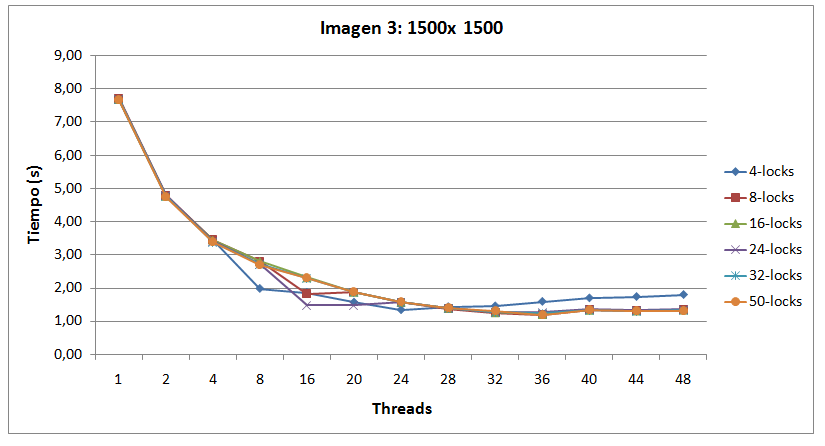
\includegraphics[width=.9\textwidth]{./imagenes/graf3-1500}
	\caption{Gr\'{a}fica de los tiempos de ejecuci\'{o}n de la imagen \ref{buena3} con un tama\~{n}o de 1500x1500}	
	\label{graf3-1500}
\end{figure}


\subsubsection{Tama\~{n}o 3000x3000}


\begin{table}[H]
	\centering
	\small
	\begin{tabular}{|c|c|c|c|c|c|c|}
		\hline
		{\bf \backslashbox{Threads}{Locks}}   & {\bf 4} & {\bf 8} & {\bf 16} & {\bf 24} & {\bf 32} & {\bf 50} \\ \hline
		{\bf Serie}  & 30,89   & 30,78   & 30,84    & 30,88    & 30,77    & 30,91    \\ \hline
		{\bf 2}  & 13,23   & 13,91   & 13,19    & 13,20    & 13,43    & 13,09    \\ \hline
		{\bf 4}  & 16,18   & 16,28   & 16,33    & 16,10    & 16,00    & 15,88    \\ \hline
		{\bf 8}  & 6,78    & 9,48    & 9,54     & 9,46     & 9,44     & 9,48     \\ \hline
		{\bf 12} & 6,80    & 7,70    & 8,98     & 7,39     & 8,96     & 8,93     \\ \hline
		{\bf 16} & 6,82    & 6,68    & 8,53     & 5,32     & 8,46     & 8,50     \\ \hline
		{\bf 20} & 5,55    & 6,77    & 6,76     & 5,42     & 6,84     & 6,85     \\ \hline
		{\bf 24} & 4,81    & 5,70    & 5,69     & 5,67     & 5,74     & 5,74     \\ \hline
		{\bf 28} & 4,89    & 4,92    & 4,96     & 4,90     & 4,97     & 4,96     \\ \hline
		{\bf 32} & 4,71    & \textbf{4,44}    & 4,51*     & 4,45*     & 4,48*     & 4,46*     \\ \hline
		{\bf 36} & 5,21    & 4,88    & 4,91     & 5,01     & 4,66     & 4,61     \\ \hline
		{\bf 40} & 5,58    & 5,02    & 5,14     & 5,00     & 5,02     & 5,08     \\ \hline
		{\bf 44} & 5,69    & 5,03    & 4,90     & 4,92     & 4,91     & 4,98     \\ \hline
		{\bf 48} & 5,96    & 4,98    & 4,84     & 4,90     & 5,01     & 4,93     \\ \hline
	\end{tabular}
	\captionsetup{justification=centering}	
	\caption{Tiempos de ejecuci\'{o}n (s) de la imagen \ref{buena3} con un tama\~{n}o de 3000x3000}
	\label{img3-3000}
\end{table}

Como se puede observar en la tabla \ref{img3-3000} el mejor resultado se consigue con 32 \textit{threads} y 8 \textit{locks}, logrando un tiempo de 4,44 segundos, un \textit{speed-up} de 6,9 y una eficiencia del 21,7\%.


\begin{figure}[H]
	\captionsetup{justification=centering}
	\centering
	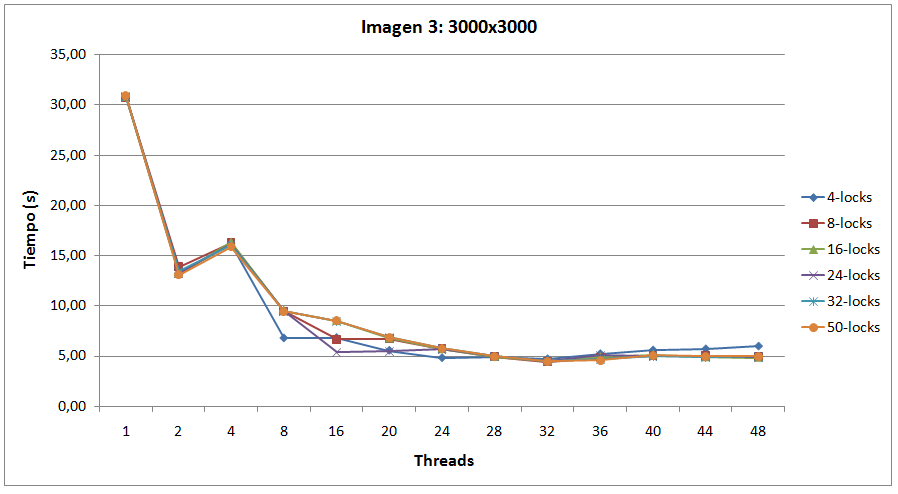
\includegraphics[width=.8\textwidth]{./imagenes/graf3-3000}
	\caption{Gr\'{a}fica de los tiempos de ejecuci\'{o}n de la imagen \ref{buena3} con un tama\~{n}o de 3000x3000}	
	\label{graf3-3000}
\end{figure}

\subsubsection{Resultado}

Los resultados de la segmentaci\'{o}n de esta tercera y \'{u}ltima imagen han sido los que se muestran en \ref{result3}, donde se ha marcado la lista $L_{out}$ de color rojo y la lista $L_{in}$ de azul. Se ha conseguido obtener el contorno las islas que es lo que se esperaba.


\begin{figure}[H]
	\captionsetup{justification=centering}
	\centering
	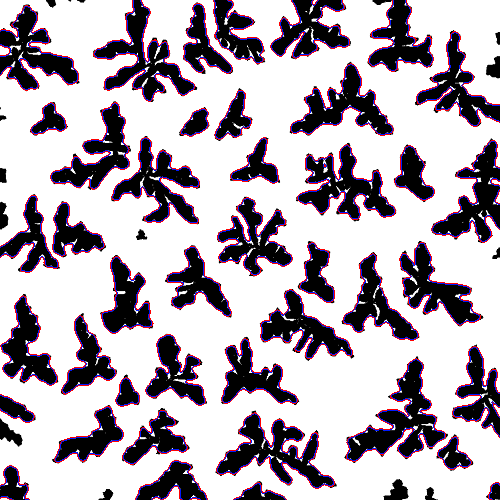
\includegraphics[width=.7\textwidth]{./imagenes/result3}
	\caption{Resultado de la segmentaci\'{o}n de la imagen \ref{buena3}}	
	\label{result3}
\end{figure}


\section{Resultados generales}


En la tabla \ref{resultadosGenerales} se puede observar un peque\~{n}o resumen de los mejores resultados obtenidos en las ejecuciones con las tres im\'{a}genes pero los tama\~{n}os m\'{a}s grandes, es decir, 3000x3000. Se ha seleccionado este tama\~{n}o ya que se puede observar mejor la paralelizaci\'{o}n realizada al tener m\'{a}s datos.

\begin{table}[H]
	\captionsetup{justification=centering}
	\centering
	\begin{tabular}{ccccc}
		\cline{2-5}
		\multicolumn{1}{l|}{}                                                           & \multicolumn{1}{c|}{{\bf Tiempo (s)}} & \multicolumn{1}{c|}{{\bf Speed-up}} & \multicolumn{1}{c|}{{\bf Threads}} & \multicolumn{1}{c|}{{\bf Locks}} \\ \hline
		\multicolumn{1}{|c|}{{\bf \begin{tabular}[c]{@{}c@{}}Imagen \\ 1\end{tabular}}} & \multicolumn{1}{c|}{6,49}         & \multicolumn{1}{c|}{6,7}            & \multicolumn{1}{c|}{48}            & \multicolumn{1}{c|}{24}          \\ \hline
		\multicolumn{1}{|c|}{{\bf \begin{tabular}[c]{@{}c@{}}Imagen\\ 2\end{tabular}}}  & \multicolumn{1}{c|}{3,85}         & \multicolumn{1}{c|}{5,7}            & \multicolumn{1}{c|}{32}            & \multicolumn{1}{c|}{32}          \\ \hline
		\multicolumn{1}{|c|}{{\bf \begin{tabular}[c]{@{}c@{}}Imagen\\ 3\end{tabular}}}  & \multicolumn{1}{c|}{4,44}         & \multicolumn{1}{c|}{6,9}            & \multicolumn{1}{c|}{32}            & \multicolumn{1}{c|}{8}            \\ \hline
		\multicolumn{1}{l}{}                                                            & \multicolumn{1}{l}{}              & \multicolumn{1}{l}{}                & \multicolumn{1}{l}{}               & \multicolumn{1}{l}{}            
	\end{tabular}
	\caption{Resultados generales obtenidos en la ejecuci\'{o}n de las tres im\'{a}genes con un tama\~{n}o de 3000x3000 \ref{buena3}}	
	\label{resultadosGenerales}	
\end{table}

Como se puede apreciar en la tabla parece ser que las im\'{a}genes dos y tres funcionan mejor ejecut\'{a}ndolas con 32 \textit{threads}. En la tercera imagen se consigue el mejor resultado con 8 \textit{locks}, sin embargo, el resultado obtenido con 32 \textit{locks} (4,48s) no se aleja mucho del \'{o}ptimo conseguido. Adem\'{a}s, en estas dos im\'{a}genes, a partir de los 32 \textit{threads} los tiempos empeoran debido al \textit{overhead} que a\~{n}ade el \textit{bus bandwidth} con tantos \textit{threads}  .

Por lo tanto, se puede generalizar en que las im\'{a}genes del mismo tipo que la segunda y la tercera funcionar\'{a}n mejor con la combinaci\'{o}n de 32 \textit{threads} y 32 \textit{locks}.

En cuanto a la primera imagen el mejor tiempo se consigue con la combinaci\'{o}n de 48 \textit{threads} y 24 \textit{locks}. Sin embargo, esta imagen tarda alrededor de 43 segundos en la versi\'{o}n serie y apenas 6,49 segundos con la mejor combinaci\'{o}n. Teniendo en cuenta \'{e}sto, a partir de los 32 \textit{threads}, el tiempo se ha reducido a alrededor de 7 segundos, reduci\'{e}ndose lentamente con m\'{a}s \textit{threads} hasta llegar a ese \'{o}ptimo de 6,49 segundos. La diferencia es apenas medio segundo, que, comparado con el tiempo en serie de 43 segundos, se tendr\'{a} que evaluar entre el coste de a\~{n}adir esos \textit{threads} y la mejora que se obtiene. Adem\'{a}s, a partir de los 24 \textit{locks} el problema de contenci\'{o}n queda resuelto. 

Como conclusi\'{o}n para los tipos de im\'{a}genes que se parezcan a la primera se puede decir que se consiguen resultados cercanos al \'{o}ptimo con 32 \textit{threads} y 24 \textit{locks}, pudiendo mejorar algo m\'{a}s invirtiendo m\'{a}s \textit{threads}.